\beginsong{Singin ja ja}

\begin{tikzpicture}[remember picture, overlay]
    \node[opacity=0.15, inner sep=0pt, anchor=north east] 
    at ([yshift=-2cm]current page text area.north east) { % Centra l'immagine nella pagina
        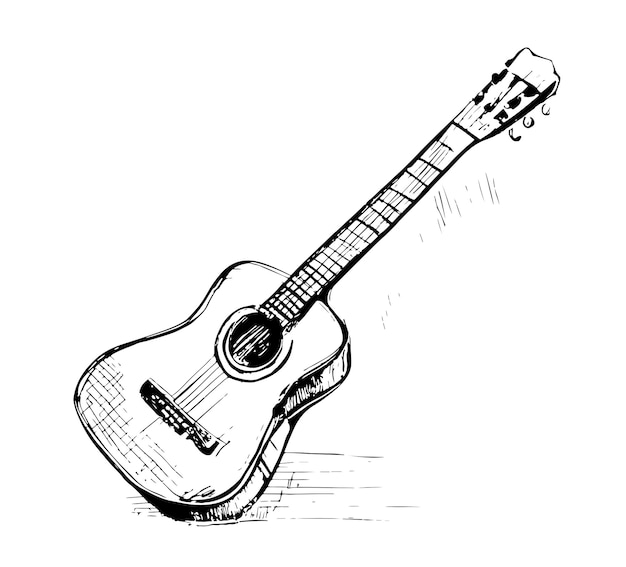
\includegraphics[width=0.35\paperwidth]{img/chitarra.png} 
    };
\end{tikzpicture}

\beginverse

Sono an\[RE]dato alla \[SOL]caccia del le\[RE]on 
\echo{pem pem!}
sono andato alla caccia del le\[LA]on 
\echo{pem pem!}
sono an\[RE]dato alla \[RE7]caccia
sono an\[SOL]dato alla \[SOL7]caccia 
sono an\[RE]dato alla \[LA]caccia del le\[RE]on \[SOL]\[RE]
\echo{pem pem!}

\endverse

\beginchorus

Singin \[RE]ja ja \[SOL]iuppy iuppy \[RE]ja ja 
Singin ja ja iuppy iuppy \[LA]jaa
singin \[RE]ja ja \[RE7]iuppy, \[SOL]ja ja 
\[SOL7]iuppy iuppy \[RE]ja ja \[LA7]iuppy iuppy \[RE]jaa \[SOL]\[RE]

\endchorus

\chordsoff

\beginverse 

Toglie l'ancora la nave per partir \echo{tu tu!} \dots

\endverse

\beginverse 

Sulla riva stan gli amici a salutar \echo{bye bye!} \dots

\endverse

\beginverse 

Siamo ormai nella foresta equatorial \echo{brr brr!} \dots

\endverse

\beginverse 

Un leone sta dormendo non lontan \echo{ronf ronf!} \dots

\endverse

\beginverse 

Se ci vede ci divora in un boccon \echo{gnam gnam!} \dots

\endverse

\beginverse 

Cari amici non facciamolo svegliar \echo{shh shh!} \dots

\endverse

\endsong
